\section{Development Frameworks}

\subsection{Programming Languages}

\subsubsection{JavaScript}

The programming language JavaScript was used for both the backend and frontend of the project. The choice was made due to its widespread use in the industry and our familiarity with the language.

JavaScript is a multi-paradigm language that is easy to learn, making it suitable for prototypes and small projects. However, it may not be the best choice for large projects or performance-intensive applications and does not offer type safety.

\textbf{Pros:}
\begin{itemize}
    \item Widely used in the industry
    \item Easy to learn
    \item Multi-paradigm language
    \item Good for small projects
    \item Good for prototyping
\end{itemize}

\textbf{Cons:}
\begin{itemize}
    \item Not suitable for large projects
    \item Not ideal for performance-intensive applications
    \item Not type-safe
\end{itemize}

\hfill \\
Although \textbf{TypeScript} offers improved type safety compared to JavaScript, it was not used in this project. The main reason was that it is more verbose, which slows down the development process.
The biggest disadvantage of JavaScript is its lack of type safety, making TypeScript a better choice for large projects. However, the trade-off of a slower development process outweighed the benefits for this project.

\subsection{Framework and Libraries}

\subsubsection{Node.js}

Node.js is a runtime environment that allows the execution of JavaScript code on the server-side. We adopted it as it is a popular and widely used framework with a large community of developers who provide useful packages and libraries through \url{https://www.npmjs.com}.

\subsubsection{Vite}

Vite is a fast build tool used for bundling our code and serving it to the browser. It is a good fit for our project as it is faster than alternatives such as Webpack and comes with a development server that features real-time updates thanks to its HMR (Hot Module Replacement) capability.

\subsubsection{React}

React is a widely used JavaScript library for developing user interfaces. It is ideal for creating prototypes as it enables the creation of fast and responsive single-page applications (SPAs). React's modular design makes it easy to create reusable components, contributing to clean and maintainable code.

\subsubsection{Tailwind CSS}

Tailwind CSS is a utility-first CSS framework that supports mobile-first, responsive design. It facilitates fast styling prototyping for the application. However, it is not a framework and does not provide reusable components. Nevertheless, it can be combined with React to create styled and reusable components.

\subsubsection{Jest}

Jest is a testing framework that enables us to test our code. It can be used to test both the backend and frontend, but we focus on testing the main functionalities of the backend. Jest also provides useful reports, including line and branch coverage.

\subsection{API}

\subsubsection{Firebase Cloud Messaging (FCM)}

Firebase Cloud Messaging (FCM) is a cross-platform messaging solution that allows us to send push notifications to our users. We use it to notify the driver when a charge has been completed.

\subsubsection{Other APIs}

Other APIs have been mocked to simulate the system's real behavior. For example, the API that retrieves the list of available DSOs for CPOs or the SMS and email API. This approach was taken as some of these APIs are not freely available, while others are unavailable altogether.
\subsection{Other Tools}
\subsubsection{Postman}
Postman is a comprehensive tool for testing and documenting APIs. It allows us to easily test our backend APIs without the need to write any client code, making it an efficient tool for development and testing purposes.

\subsubsection{Docker}
Docker is a powerful tool for creating and managing containers, which can be used to run applications in a production environment. We have chosen to use Docker in our project as it provides an easy and reliable way to deploy the application, while also reducing inconsistencies between different operating systems. With Docker, it is possible to easily manage the backend and frontend of our application in a containerized environment.
\begin{figure}[H]
    \centering
    \hspace*{-2cm}
    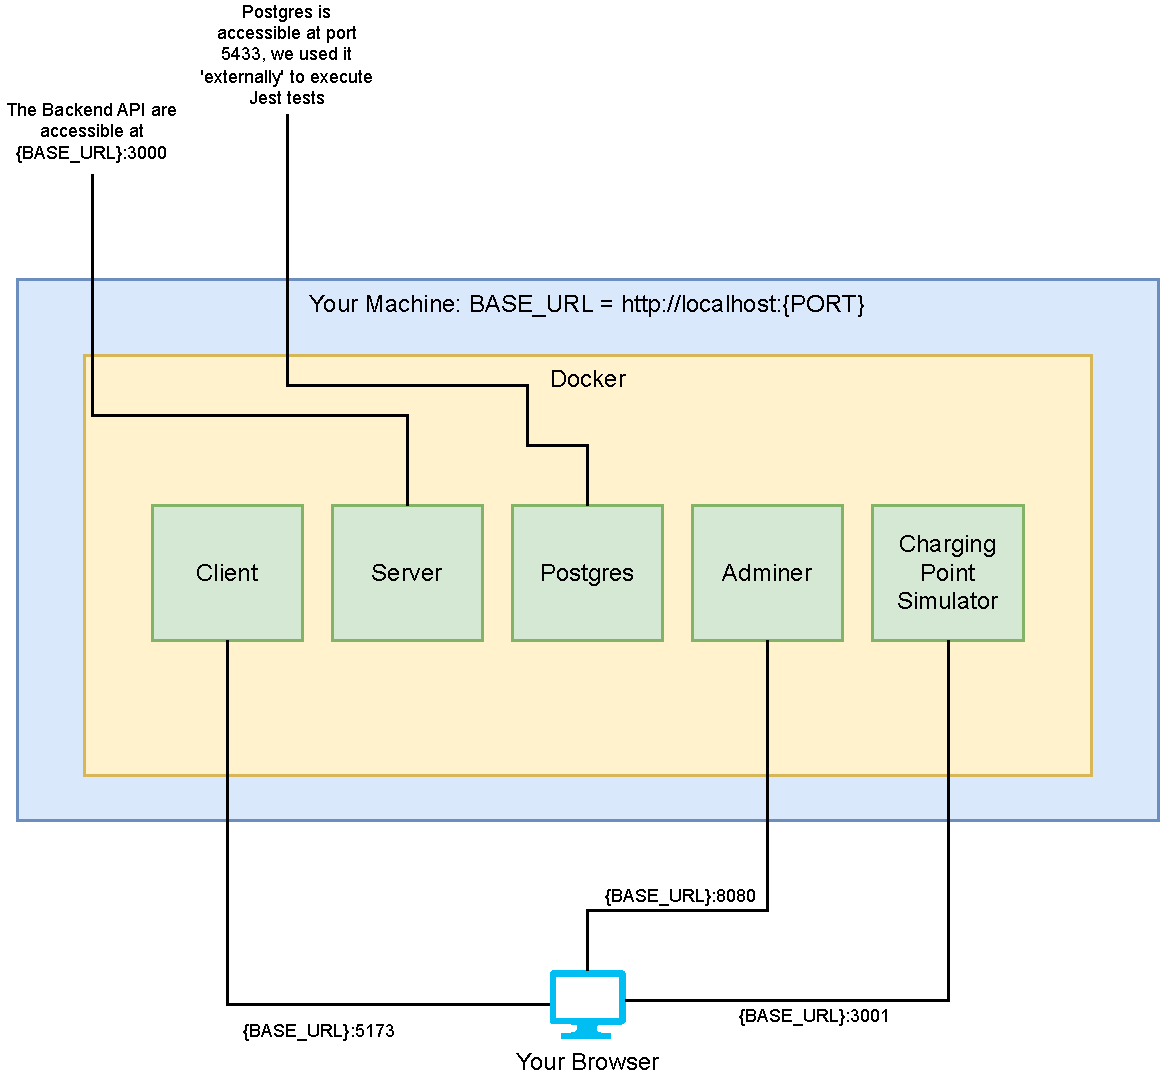
\includegraphics[scale=0.60]{src/docker_structure/docker_structure.pdf}
    \caption{Internal structure of the container.}
\end{figure}

\subsubsection{Jsdoc}
Jsdoc is a tool used to document our JavaScript code. It helps to generate clear, comprehensive and well-organized documentation of the backend of our application. This ensures that the code is easy to understand and maintain, especially for other developers who may work on the project in the future. With Jsdoc, we can also provide information such as function signatures, parameter descriptions, and return types, making it easier to use and debug the code.
\hfill \\ The generated documentation is in the /docs folder of the server.
